\chapter{Interprocess Communication}

\todo{Epigraph}

In very simple embedded systems and early computers, processes directly access memory i.e. ``Address 1234'' corresponds to a particular byte stored in a particular part of physical memory. For example the IBM 709 had to read and write directly to a tape with no level of abstraction \cite[P. 65]{ibm709}. Even in systems after that, it was hard to adopt virtual memory because virtual memory required the whole fetch cycle to be altered through hardware -- a change many manufacturers still thought was expensive. In the PDP-10, a workaround was used by using different registers for each process and then virtual memory was added later. In modern systems, this is no longer the case. Instead each process is isolated, and there is a translation process between the address of a particular CPU instruction or piece of data of a process and the actual byte of physical memory (``RAM''). Memory addresses no longer map to physical addresses; the process runs inside virtual memory. Virtual memory not only keeps processes safe (because one process cannot directly read or modify another process's memory) it also allows the system to efficiently allocate and re-allocate portions of memory to different processes. The modern process of translating memory is as follows.

\begin{enumerate}
\item A process makes a memory request
\item The circuit first checks the Translation Lookaside Buffer (TLB) if the address page is cached into memory. It skips to the reading from/writing to phase if found otherwise the request goes to the MMU.
\item The Memory Management Unit (MMU) performs the address translation. If the translation succeeds (more on that later), the page get pulled from RAM -- conceptually the entire page isn't loaded up. The result is cached in the TLB. 
\item The CPU performs the operation by either reading from the physical address or writing to the address.
\end{enumerate}

\section{MMU and Translating Addresses}

The Memory Management Unit is part of the CPU, and it converts a virtual memory address into a physical address. There is a sort of pseudocode associated with the MMU.

\begin{enumerate}
\item Receive address
\item Try to translate address according to the programmed scheme
\item If the translation fails, report an invalid address
\item Otherwise,
	\begin{enumerate}
	\item If the page exists in memory, check if the process has permissions
		to perform the operation on the page meaning the process has access
		to the page, and it is reading from the page/writing to a page
		that is not marked as read only.
		\begin{enumerate}
		\item If so then provide the address, cache the results in the TLB
		\item Otherwise trigger a hardware interrupt. The kernel 
			will most likely send a SIGSEGV or a Segmentation Violation.
		\end{enumerate}
	\item If the page doesn't exist in memory, generate an Interrupt.
		\begin{enumerate}
		\item The kernel could realize that this page could either be not
			allocated or on disk. If it fits the mapping, allocate the page
			and try the operation again.
		\item Otherwise, this is an invalid access and the kernel will most
			likely send a SIGSEGV to the process.
		\end{enumerate}
	\end{enumerate}
\end{enumerate}

Imagine you had a 32 bit machine, meaning pointers are 32 bits. They can address $2^{32}$ different locations or 4GB of memory where one address is one byte. Imagine we had a large table - here's the clever part - stored in memory! For every possible address (all 4 billion of them) we will store the `real' i.e. ~physical address. Each physical address will need 4 bytes (to hold the 32 bits). This scheme would require 16 billion bytes to store all of entries. Oops - our lookup scheme would consume all of the memory that we could possibly buy for our 4GB machine. We need to do better than this. Our lookup table better be smaller than the memory we have otherwise we will have no space left for our actual programs and operating system data. The solution is to chunk memory into small regions called `pages' and `frames' and use a lookup table for each page.

A \textbf{page} is a block of virtual memory. A typical block size on Linux operating system is 4KB or $2^{12}$ addresses, though you can find examples of larger blocks. So rather than talking about individual bytes we can talk about blocks of 4KBs, each block is called a page. We can also number our pages (``Page 0'' ``Page 1'' etc). Let's do a sample calculation of how many pages are there assume page size of 4KB.

\begin{shaded*}
For a 32 bit machine, $2^{32}$ address / $2^{12}$ (address/page) = $2^{20}$ pages.

For a 64 bit machine, $2^{64}$ / $2^{12}$ = $2^{52}$, which is roughly $10^{15}$ pages.
\end{shaded*}

\subsection{Terminology}

A \textbf{frame} (or sometimes called a `page frame') is a block of \emph{physical memory} or RAM (=Random Access Memory). This kind of memory is occasionally called `primary storage' in contrast with lower, secondary storage such as spinning disks that have lower access times. A frame is the same number of bytes as a virtual page. If a 32 bit machine has $2^{32} B$ of RAM, then there will be the same number of them in the addressable space of the machine. It's unlikely that a 64 bit machine will ever have $2^{64}$ bytes of RAM.

A \textbf{page table} is a mapping between a page to the frame. For example Page 1 might be mapped to frame 45, page 2 mapped to frame 30. Other frames might be currently unused or assigned to other running processes, or used internally by the operating system.

A simple page table could be imagined as an array.
\begin{lstlisting}[language=C]
int frame_num = table[page_num]; 
\end{lstlisting}

For a 32 bit machine with 4KB pages, each entry needs to hold a frame number - i.e.~20 bits because we calculated there are $2^{20}$ frames. That's 2.5 bytes per entry! In practice, we'll round that up to 4 bytes per entry and find a use for those spare bits. With 4 bytes per entry x $2^{20}$ entries = 4 MB of physical memory are required to hold the page table 
For a 64 bit machine with 4KB pages, each entry needs 52 bits. Let's round up to 64 bits (8 bytes) per entry. With $2^{52}$ entries thats $2^{55}$ bytes (roughly 40 peta bytes\ldots{}) Oops our page table is too large 
In 64 bit architectures memory addresses are sparse, so we need a mechanism to reduce the page table size, given that most of the entries will never be used.

\begin{wrapfig}
% 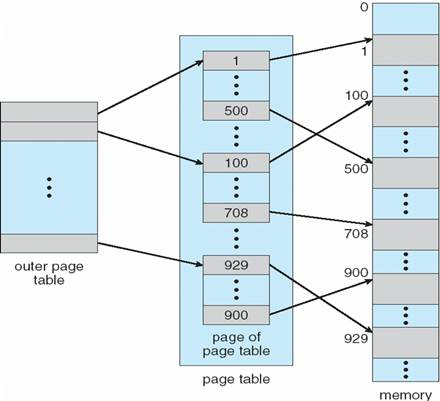
\includegraphics{ipc/images/page_table1.jpg}
\end{wrapfig}

An \textbf{offset} take a particular page and looks up a byte by adding it to the start of the page. Remember our page table maps pages to frames, but each page is a block of contiguous addresses. How do we calculate which particular byte to use inside a particular frame? The solution is to re-use the lowest bits of the virtual memory address directly. For example, suppose our process is reading the following address- \keyword{VirtualAddress = 11110000111100001111000010101010 (binary)}

On a machine with page size 256 Bytes, then the lowest 8 bits (10101010) will be used as the offset. The remaining upper bits will be the page number (111100001111000011110000).

\subsection{Multi-level page tables}\label{multi-level-page-tables}
 Multi-level pages are one solution to the page table size issue for 64 bit architectures. We'll look at the simplest implementation - a two level page table. Each table is a list of pointers that point to the next level of tables, not all sub-tables need to exist. An example, two level page table for a 32 bit architecture is shown below-

\begin{verbatim}
VirtualAddress = 11110000111111110000000010101010 (binary)
                 |-Index1-||        ||          | 10 bit Directory index
                           |-Index2-||          | 10 bit Sub-table index
                                     |--offset--| 12 bit offset (passed directly to RAM)
\end{verbatim}

 In the above scheme, determining the frame number requires two memory reads: The topmost 10 bits are used in a directory of page tables. If 2 bytes are used for each entry, we only need 2KB to store this entire directory. Each subtable will point to physical frames (i.e.~required 4 bytes to store the 20 bits). However, for processes with only tiny memory needs, we only need to specify entries for low memory address (for the heap and program code) and high memory addresses (for the stack). Each subtable is 1024 entries x 4 bytes i.e.~4KB for each subtable.

 Thus the total memory overhead for our multi-level page table has shrunk from 4MB (for the single level implementation) to 3 frames of memory (12KB) ! Here's why: We need at least one frame for the high level directory and two frames for just two sub-tables. One sub-table is necessary for the low addresses (program code, constants and possibly a tiny heap), the other sub-table is for higher addresses used by the environment and stack. In practice, real programs will likely need more sub-table entries, as each subtable can only reference 1024*4KB = 4MB of address space but the main point still stands - we have significantly reduced the memory overhead required to perform page table look ups.

\subsection{Page Table Disadvantages}
 Yes - Significantly ! (But thanks to clever hardware, usually no\ldots{}) Compared to reading or writing memory directly. For a single page table, our machine is now twice as slow! (Two memory accesses are required) For a two-level page table, memory access is now three times as slow. (Three memory accesses are required)

 To overcome this overhead, the MMU includes an associative cache of recently-used virtual-page-to-frame lookups. This cache is called the TLB (``translation lookaside buffer''). Everytime a virtual address needs to be translated into a physical memory location, the TLB is queried in parallel to the page table. For most memory accesses of most programs, there is a significant chance that the TLB has cached the results. However if a program does not have good cache coherence (for example is reading from random memory locations of many different pages) then the TLB will not have the result cache and now the MMU must use the much slower page table to determine the physical frame.

\begin{wrapfig}
% 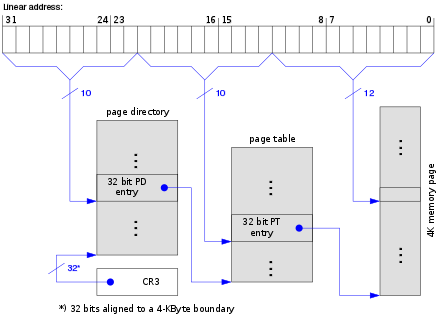
\includegraphics{ipc/images/440px-X86_Paging_4K.png}
\end{wrapfig}

This may be how one splits up a multi level page table.

\section{Advanced Frames and Page Protections}\label{advanced-frames-and-page-protections}

Frames be shared between processes! In addition to storing the frame number, the page table can be used to store whether a process can write or only read a particular frame. Read only frames can then be safely shared between multiple processes. For example, the C-library instruction code can be shared between all processes that dynamically load the code into the process memory. Each process can only read that memory. Meaning that if you try to write to a read-only page in memory you will get a \keyword{SEGFAULT}. That is why sometimes memory accesses segfault and sometimes they don't, it all depends on if your hardware says that you can access.

In addition, processes can share a page with a child process using the \keyword{mmap} system call. \keyword{mmap} is an interesting call because instead of tying each virtual address to a physical frame, it ties it to something else. That something else can be a file, a GPU unit, or any other memory mapped operation that you can think of! Writing to the memory address may write through to the device or the write may be paused by the operating system but this is a very powerful abstraction because often the operating system is able to perform optimizations (multiple processes memory mapping the same file can have the kernel create one mapping). In addition, it is common to store at least read-only, modification and execution information.

\subsubsection{Read-only bit}
The read-only bit marks the page as read-only. Attempts to write to the page will cause a page fault. The page fault will then be handled by the Kernel. Two examples of the read-only page include sharing the c runtime library between multiple processes (for security you wouldn't want to allow one process to modify the library); and Copy-On-Write where the cost of duplicating a page can be delayed until the first write occurs.

\subsubsection{Dirty bit}

\href{http://en.wikipedia.org/wiki/Page\_table\#Page\_table\_data}{Page Table} The dirty bit allows for a performance optimization. A page on disk that is paged in to physical memory, then read from, and subsequently paged out again does not need to be written back to disk, since the page hasn't changed. However, if the page was written to after it's paged in, its dirty bit will be set, indicating that the page must be written back to the backing store. This strategy requires that the backing store retain a copy of the page after it is paged in to memory. When a dirty bit is not used, the backing store need only be as large as the instantaneous total size of all paged-out pages at any moment. When a dirty bit is used, at all times some pages will exist in both physical memory and the backing store.

\subsubsection{Execution bit}\label{execution-bit}
The execution bit defines whether bytes in a page can be executed as CPU instructions. By disabling a page, it prevents code that is maliciously stored in the process memory (e.g.~by stack overflow) from being easily executed. (further reading: \href{http://en.wikipedia.org/wiki/NX\_bit\#Hardware\_background}{background})

\subsection{Page Faults}

 A page fault is when a running program tries to access some virtual memory in its address space that is not mapped to physical memory. Page faults will also occur in other situations. There are three types of Page Faults

\begin{enumerate}
 \item \textbf{Minor} If there is no mapping yet for the page, but it is a valid address. This could be memory asked for by \keyword{sbrk(2)} but not written to yet meaning that the operating system can wait for the first write before allocating space. The OS simply makes the page, loads it into memory, and moves on.

 \item \textbf{Major} If the mapping to the page is not in memory but on disk. What this will do is swap the page into memory and swap another page out. If this happens frequently enough, your program is said to \emph{thrash} the MMU.

 \item \textbf{Invalid} When you try to write to a non-writable memory address or read to a non-readable memory address. The MMU generates an invalid fault and the OS will usually generate a \keyword{SIGSEGV} meaning segmentation violation meaning that you wrote outside the segment that you could write to.
\end{enumerate}

\section{Pipes}

Inter process communication is any way for one process to talk to another process. You've already seen one form of this virtual memory! A piece of virtual memory can be shared between parent and child, leading to communication. You may want to wrap that memory in \keyword{pthread\_mutexattr\_setpshared(\&attrmutex,\ PTHREAD\_PROCESS\_SHARED);} mutex (or a process wide mutex) to prevent race conditions. There are more standard ways of IPC, like pipes! Consider if you type the following into your terminal.

\begin{verbatim}
$ ls -1 | cut -d'.' -f1 | uniq | sort | tee dir_contents
\end{verbatim}

What does the following code do? Well it \keyword{ls}'s the current directory (the -1 means that it outputs one entry per line). The \keyword{cut} command then takes everything before the first period. Uniq makes sure all the lines are uniq, sort sorts them and tee outputs to a file. The important part is that bash creates \textbf{5 separate processes} and connects their standard outs/stdins with pipes the trail lookssomething like this.

\begin{verbatim}
(0) ls (1)------>(0) cut (1)------->(0) uniq (1)------>(0) sort (1)------>(0) tee (1)
\end{verbatim}

The numbers in the pipes are the file descriptors for each process and the arrow represents the redirect or where the output of the pipe is going. A POSIX pipe is almost like its real counterpart - you can stuff bytes down one end and they will appear at the other end in the same order. Unlike real pipes however, the flow is always in the same direction, one file descriptor is used for reading and the other for writing. The \keyword{pipe} system call is used to create a pipe. These file descriptors can be used with \keyword{read} and with \keyword{write}. A common method of using pipes is to create the pipe before forking in order to communicate with a child process

\begin{lstlisting}[language=C]
int filedes[2];
pipe (filedes);
pid_t child = fork();
if (child > 0) { /* I must be the parent */
    char buffer[80];
    int bytesread = read(filedes[0], buffer, sizeof(buffer));
    // do something with the bytes read    
} else {
	write(filedes[1], "done", 4);
}
\end{lstlisting}

One can use pipes inside of the same process, but there tends to be no added benefit. Here's an example program that sends a message to itself:

\begin{lstlisting}[language=C]
#include <unistd.h>
#include <stdlib.h>
#include <stdio.h>

int main() {
    int fh[2];
    pipe(fh);
    FILE *reader = fdopen(fh[0], "r");
    FILE *writer = fdopen(fh[1], "w");
    // Hurrah now I can use printf rather than using low-level read() write()
    printf("Writing...\n");
    fprintf(writer,"%d %d %d\n", 10, 20, 30);
    fflush(writer);
    
    printf("Reading...\n");
    int results[3];
    int ok = fscanf(reader,"%d %d %d", results, results + 1, results + 2);
    printf("%d values parsed: %d %d %d\n", ok, results[0], results[1], results[2]);
    
    return 0;
}
\end{lstlisting}

The problem with using a pipe in this fashion is that writing to a pipe can block meaning the pipe only has a limited buffering capacity. If the pipe is full the writing process will block! The maximum size of the buffer is system dependent; typical values from 4KB upto 128KB.

\begin{lstlisting}[language=C]
int main() {
    int fh[2];
    pipe(fh);
    int b = 0;
    #define MESG "..............................."
    while(1) {
        printf("%d\n",b);
        write(fh[1], MESG, sizeof(MESG))
        b+=sizeof(MESG);
    }
    return 0;
}
\end{lstlisting}

\subsection{Pipe Gotchas}\label{pipe-gotchas}

Here's a complete example that doesn't work! The child reads one byte at a time from the pipe and prints it out - but we never see the message! Can you see why?

\begin{lstlisting}[language=C]
#include <stdio.h>
#include <stdlib.h>
#include <unistd.h>
#include <signal.h>

int main() {
    int fd[2];
    pipe(fd);
    //You must read from fd[0] and write from fd[1]
    printf("Reading from %d, writing to %d\n", fd[0], fd[1]);

    pid_t p = fork();
    if (p > 0) {
        /* I have a child therefore I am the parent*/
        write(fd[1],"Hi Child!",9);

        /*don't forget your child*/
        wait(NULL);
    } else {
        char buf;
        int bytesread;
        // read one byte at a time.
        while ((bytesread = read(fd[0], &buf, 1)) > 0) {
            putchar(buf);
        }
    }
    return 0;
}
\end{lstlisting}

The parent sends the bytes \keyword{H,i,(space),C...!} into the pipe (this may block if the pipe is full). The child starts reading the pipe one byte at a time. In the above case, the child process will read and print each character. However it never leaves the while loop! When there are no characters left to read it simply blocks and waits for more 

The call \keyword{putchar} writes the characters out but we never flush the \keyword{stdout} buffer. i.e.~We have transferred the message from one process to another but it has not yet been printed. To see the message we could flush the buffer e.g. \keyword{fflush(stdout)} (or \keyword{printf("\textbackslash{}n")} if the output is going to a terminal). A better solution would also exit the loop by checking for an end-of-message marker,

\begin{lstlisting}[language=C]
        while ((bytesread = read(fd[0], &buf, 1)) > 0) {
            putchar(buf);
            if (buf == '!') break; /* End of message */
        }
\end{lstlisting}

Processes receive the signal SIGPIPE when no process is listening! From
the pipe(2) man page -

\begin{lstlisting}[language=C]
If all file descriptors referring to the read end of a pipe have been closed,
 then a write(2) will cause a SIGPIPE signal to be generated for the calling process. 
\end{lstlisting}

Tip: Notice only the writer (not a reader) can use this signal. To
inform the reader that a writer is closing their end of the pipe, you
could write your own special byte (e.g.~0xff) or a message (
\keyword{"Bye!"})

Here's an example of catching this signal that does not work! Can you
see why?

\begin{lstlisting}[language=C]
#include <stdio.h>
#include <stdio.h>
#include <unistd.h>
#include <signal.h>

void no_one_listening(int signal) {
    write(1, "No one is listening!\n", 21);
}

int main() {
    signal(SIGPIPE, no_one_listening);
    int filedes[2];
    
    pipe(filedes);
    pid_t child = fork();
    if (child > 0) { 
        /* I must be the parent. Close the listening end of the pipe */
        /* I'm not listening anymore!*/
        close(filedes[0]);
    } else {
        /* Child writes messages to the pipe */
        write(filedes[1], "One", 3);
        sleep(2);
        // Will this write generate SIGPIPE ?
        write(filedes[1], "Two", 3);
        write(1, "Done\n", 5);
    }
    return 0;
}
\end{lstlisting}

The mistake in above code is that there is still a reader for the pipe! The child still has the pipe's first file descriptor open and remember the specification? All readers must be closed 

When forking, \emph{It is common practice} to close the unnecessary (unused) end of each pipe in the child and parent process. For example the parent might close the reading end and the child might close the writing end (and vice versa if you have two pipes)

\subsection{Why is my pipe hanging?}\label{why-is-my-pipe-hanging}

Reads and writes hang on Named Pipes until there is at least one reader and one writer, take this

\begin{lstlisting}[language=C]
1$ mkfifo fifo
1$ echo Hello > fifo
# This will hang until I do this on another terminal or another process
2$ cat fifo
Hello
\end{lstlisting}

Any \keyword{open} is called on a named pipe the kernel blocks until another process calls the opposite open. Meaning, echo calls \keyword{open(..,\ O\_RDONLY)} but that blocks until cat calls \keyword{open(..,\ O\_WRONLY)}, then the programs are allowed to continue.

\subsection{Race condition with named pipes}

What is wrong with the following program?

\begin{lstlisting}[language=C]
//Program 1

int main(){
    int fd = open("fifo", O_RDWR | O_TRUNC);
    write(fd, "Hello!", 6);
    close(fd);
    return 0;
}

//Program 2
int main() {
    char buffer[7];
    int fd = open("fifo", O_RDONLY);
    read(fd, buffer, 6);
    buffer[6] = '\0';
    printf("%s\n", buffer);
    return 0;
}
\end{lstlisting}

This may never print hello because of a race condition. Since you opened the pipe in the first process under both permissions, open won't wait for a reader because you told the operating system that you are a reader! Sometimes it looks like it works because the execution of the code looks something like this.

\begin{enumerate}
\item Process 1: open(O\_RDWR) \& write()
\item Process 2: open(O\_RDONLY) \& read()
\item Process 1: close() \& exit()
\item Process 2: print() \& exit()
\end{enumerate}

\begin{enumerate}
\item Process 1: open(O\_RDWR) \& write()
\item Process 1: close() \& exit()
\item Process 2: open(O\_RDONLY) (Blocks indefinitely) 
\end{enumerate}

\subsection{What is filling up the pipe? What happens when the pipe
becomes
full?}\label{what-is-filling-up-the-pipe-what-happens-when-the-pipe-becomes-full}
 A pipe gets filled up when the writer writes too much to the pipe without the reader reading any of it. When the pipes become full, all writes fail until a read occurs. Even then, a write may partial fail if the pipe has a little bit of space left but not enough for the entire message 

 To avoid this, usually two things are done. Either increase the size of the pipe. Or more commonly, fix your program design so that the pipe is constantly being read from.

\subsection{Are pipes process safe?}\label{are-pipes-process-safe}

 Yes! Pipe write are atomic up to the size of the pipe. Meaning that if two processes try to write to the same pipe, the kernel has internal mutexes with the pipe that it will lock, do the write, and return. The only gotcha is when the pipe is about to become full. If two processes are trying to write and the pipe can only satisfy a partial write, that pipe write is not atomic -- be careful about that!

\subsection{The lifetime of pipes}\label{the-lifetime-of-pipes}
 Unnamed pipes (the kind we've seen up to this point) live in memory (do not take up any disk space) and are a simple and efficient form of inter-process communication (IPC) that is useful for streaming data and simple messages. Once all processes have closed, the pipe resources are freed.


\subsection{Want to use pipes with printf and scanf? Use fdopen!}

 POSIX file descriptors are simple integers 0,1,2,3\ldots{} At the C library level, C wraps these with a buffer and useful functions like printf and scanf, so we that we can easily print or parse integers, strings etc. If you already have a file descriptor then you can `wrap' it yourself into a FILE pointer using \keyword{fdopen} :

\begin{lstlisting}[language=C]
#include <sys/types.h>
#include <sys/stat.h>
#include <fcntl.h>

int main() {
    char *name="Fred";
    int score = 123;
    int filedes = open("mydata.txt", "w", O_CREAT, S_IWUSR | S_IRUSR);

    FILE *f = fdopen(filedes, "w");
    fprintf(f, "Name:%s Score:%d\n", name, score);
    fclose(f);
\end{lstlisting}

For writing to files this is unnecessary - just use \keyword{fopen} which does the same as \keyword{open} and \keyword{fdopen} However for pipes, we already have a file descriptor - so this is great time to use \keyword{fdopen} 

Here's a complete example using pipes that almost works! Can you spot the error? Hint: The parent never prints anything!

\begin{lstlisting}[language=C]
#include <unistd.h>
#include <stdlib.h>
#include <stdio.h>

int main() {
    int fh[2];
    pipe(fh);
    FILE *reader = fdopen(fh[0], "r");
    FILE *writer = fdopen(fh[1], "w");
    pid_t p = fork();
    if (p > 0) {
        int score;
        fscanf(reader, "Score %d", &score);
        printf("The child says the score is %d\n", score);
    } else {
        fprintf(writer, "Score %d", 10 + 10);
        fflush(writer);
    }
    return 0;
}
\end{lstlisting}

Note the unnamed pipe resource will disappear once both the child and parent have exited. In the above example the child will send the bytes and the parent will receive the bytes from the pipe. However, no end-of-line character is ever sent, so \keyword{fscanf} will continue to ask for bytes because it is waiting for the end of the line i.e.~it will wait forever! The fix is to ensure we send a newline character, so that \keyword{fscanf} will return.

\begin{lstlisting}[language=C]
change:   fprintf(writer, "Score %d", 10 + 10);
to:       fprintf(writer, "Score %d\n", 10 + 10);
\end{lstlisting}

If you want your bytes to be sent to the pipe immediately, you'll need to fflush! At the beginning of this course we assumed that file streams are always \emph{line buffered} i.e.~the C library will flush its buffer everytime you send a newline character. Actually this is only true for terminal streams - for other filestreams the C library attempts to improve performance by only flushing when it's internal buffer is full or the file is closed.

\subsection{When do I need two pipes?}

If you need to send data to and from a child asynchronously, then two pipes are required (one for each direction). Otherwise the child would attempt to read its own data intended for the parent (and vice versa)!

\section{Named Pipes}\label{named-pipes}

\subsection{How do I create named pipes?}\label{how-do-i-create-named-pipes}

An alternative to \emph{unamed} pipes is \emph{named} pipes created using \keyword{mkfifo}.

From the command line: \keyword{mkfifo} From C: \keyword{int\ mkfifo(const\ char\ *pathname,\ mode\_t\ mode);}

You give it the path name and the operation mode, it will be ready to go! Named pipes take up no space on the disk. What the operating system is essentially telling you when you have a named pipe is that it will create an unnamed pipe that refers to the named pipe, and that's it! There is no additional magic. This is just for programming convenience if processes are started without forking (meaning that there would be no way to get the file descriptor to the child process for an unnamed pipe)


\subsection{Two types of files}

 On linux, there are two abstractions with files. The first is the linux \keyword{fd} level abstraction.

 \begin{itemize}
\item \keyword{open} takes a path to a file and creates a file descriptor entry in the process table. If the file is not available to you, it errors out.
\item \keyword{read} takes a number of bytes that the kernel has received and reads them into a user space buffer. If the file is not open in read mode, this will break.
\item \keyword{write} outputs a number of bytes to a file descriptor. If the file is not open in write mode, this will break. This may be buffered internally.
\item \keyword{close} removes a file descriptor from a process' file descriptors. This always succeeds on a valid file descriptor.
\item \keyword{lseek} takes a file descriptor and moves it to a certain position. Can fail if the seek is out of bounds.
\item \keyword{fcntl} is the catch all function for file descriptors. You can do everything with this function. Set file locks, read, write, edit permissions, etc \ldots{}
\item \ldots{}
 \end{itemize}

 And so on. The linux interface is very powerful and expressive, but sometimes we need portability (for example if we are writing for a mac or windows). This is where C's abstraction comes into play. On different operating systems, C uses the low level functions to create a wrapper around files you can use everywhere, meaning that C on linux uses the above calls.

\begin{itemize}
\item \keyword{fopen} opens a file and returns an object. \keyword{null} is returned if you don't have permission for the file.
\item \keyword{fread} reads a certain number of bytes from a file. An error is returned if already at the end of file when which you must call \keyword{feof()} in order to check.
\item \keyword{fgetc/fgets}
\item \keyword{fscanf} 
\item \keyword{fwrite} 
\item \keyword{fprintf} 
\item \keyword{fclose} 
\item \keyword{fflush}
\end{itemize}

 But you don't get the expressiveness that linux gives you with system calls you can convert back and forth between them with \keyword{int\ fileno(FILE*\ stream)} and \keyword{FILE*\ fdopen(int\ fd...)} 

 Another important aspect to note is the C files are \textbf{buffered} meaning that their contents may not be written right away by default. You can can change that with C options.

\subsection{How do I tell how large a file is?}\label{how-do-i-tell-how-large-a-file-is}

For files less than the size of a long, using fseek and ftell is a
simple way to accomplish this:

Move to the end of the file and find out the current position.

\begin{lstlisting}[language=C]
fseek(f, 0, SEEK_END);
long pos = ftell(f);
\end{lstlisting}

This tells us the current position in the file in bytes - i.e.~the
length of the file!

\keyword{fseek} can also be used to set the absolute position.

\begin{lstlisting}[language=C]
fseek(f, 0, SEEK_SET); // Move to the start of the file 
fseek(f, posn, SEEK_SET);  // Move to 'posn' in the file.
\end{lstlisting}

All future reads and writes in the parent or child processes will honor
this position. Note writing or reading from the file will change the
current position.

See the man pages for fseek and ftell for more information.

\subsection{But try not to do this}

\textbf{Note: This is not recommended in the usual case because of a quirk with the C language}. That quirk is that longs only need to be \textbf{4 Bytes big} meaning that the maximum size that \keyword{ftell} can return is a little under 2 Gigabytes (which we know nowadays our files could be hundreds of gigabytes or even terabytes on a distributed file system). What should we do instead? Use \keyword{stat}! We will cover stat in a later part but here is some code that will tell you the size of the file

\begin{lstlisting}[language=C]
struct stat buf;
if(stat(filename, &buf) == -1){
    return -1;
}
return (ssize_t)buf.st_size;
\end{lstlisting}

\keyword{buf.st\_size} is of type \keyword{off\_t} which is big enough for large files.

\subsection{What happens if a child process closes a filestream using fclose or close?}

Closing a file stream is unique to each process. Other processes can continue to use their own file-handle. Remember, everything is copied over when a child is created, even the relative positions of the files.

\subsection{How about mmap for files?}\label{how-about-mmap-for-files}

One of the general uses for mmap is to map a file to memory. This does not mean that the file is malloc'ed to memory right away. Take the following code for example.

\begin{lstlisting}[language=C]
int fd = open(...); //File is 2 Pages
char* addr = mmap(..fd..);
addr[0] = 'l';
\end{lstlisting}

 The kernel may say, ``okay I see that you want to mmap the file into memory, so I'll reserve some space in your address space that is the length of the file''. That means when you write to addr{[}0{]} that you are actually writing to the first byte of the file. The kernel can actually do some optimizations too. Instead of loading the file into memory, it may only load pages at a time because if the file is 1024 pages; you may only access 3 or 4 pages making loading the entire file a waste of time. That is why page faults are so powerful! They let the operating system take control of how much you use your files.

\subsection{For every mmap}

 Remember that once you are done \keyword{mmap}ping that you \keyword{munmap} to tell the operating system that you are no longer using the pages allocated, so the OS can write it back to disk and give you the addresses back in case you need to malloc later.

\bibliographystyle{plainnat}
\bibliography{ipc/ipc}
